\chapter{
  The LHC and CMS Experiment
 }\label{ch_cms}

The physics analysis is carried out using data collected by the \gls{CMS} experiment at
\gls{CERN} \gls{LHC} accelerator. This chapter provides overview of the \gls{LHC}
and details of the CMS experiment and its sub-detectors for particle tracking
and calorimetry.

\section{
  The Large Hadron Collider
 }\label{ch_cms:lhc}

The \gls{LHC} is the largest proton-proton
collider, located at
\gls{CERN} in Geneva, Switzerland.
The main \gls{LHC} ring is 27\km{} in circumference
and 50 to 175\m{} underground.
The \gls{LHC} is built to collide protons at 14\TeV{} center-of-mass energy,
LHC delivered proton-proton collisions at 7 and 8\TeV{}
during run1 (2010--2012), and at 13\TeV{} center-of-mass energy during
run2 (2015--2018)
~\cite{Evans:2008}.

Figure~\ref{fig:lhc} describes \gls{CERN} accelerator complex.
The protons are sourced by ionizing hydrogen atoms
and then fed into a \gls{LINAC}.
The \gls{LINAC} accelerates the protons to 50\MeV{} and delivers them to the booster.
Then the booster increases the energy of the protons to 1.4\GeV{} and
feeds them to the \gls{PS} which further increases their energy to 25\GeV{}
and starts bunching them together with bunches 25\nanoseconds{} apart.
The proton bunches are passed through \gls{SPS} which brings their energy
to 450\GeV{} and bunches are then finally sent to main \gls{LHC} clockwise and counterclockwise
rings where they are accelerated to final energy required which is 6.5\TeV{}
for both bunches going clockwise and counterclockwise
to obtain collisions at 13\TeV{} center-of-mass energy.

The proton-proton collisions occurs, at four different locations where two
general purpose detectors \gls{CMS} and \gls{ATLAS}, and
two specific purpose detector \gls{ALICE} and \gls{LHCb} are located.

\begin{figure}[!ht]
  \centering
  \includegraphics[width=0.98\textwidth]{figures/lhc-scheme.png}
  \caption[A schematic of the CERN accelerator complex]%
  {A schematic of the CERN accelerator complex~\cite{image-lhc-scheme}}%
  \label{fig:lhc}
\end{figure}

\subsection{
  Integrated Luminosity
}\label{ch_cms:cms-lumi}

Luminosity is a measure of how many events can happen per unit area and per
unit time for a collision or scattering process, and it is defined as,
%
\begin{equation}
  L = \frac{1}{\sigma} \frac{dN}{dt}, \quad L_{\text{int}} = \int L dt
\end{equation}

where \(\sigma \) is cross-section of the process
and \(L\) is the instantaneous luminosity (\( \cm{}^{-2} \seconds^{-1} \)),
and \( L_{\text{int}} \) is the integrated luminosity usually
expressed in inverse units of cross-section (\pbinv{}, \fbinv{}, etc.).

For proton-proton collision at \gls{LHC}
the nominal instantaneous luminosity is of the order of \( 10^{34} \cm{}^{-2} \seconds^{-1}\),
and integrated luminosity delivered and recorded by \gls{CMS} during run2\footnote{2\textsuperscript{nd} run period (2015--2018) of proton-proton collisions at LHC} operation
is shown in Figure~\ref{fig:int-lumi}.

\begin{figure}[!ht]
  \centering
  \includegraphics[width=0.60\textwidth]{figures/int_lumi_pp_run2.pdf}
  \caption[Integrated delivered and recorded luminosity
    for 2015--2018 proton-proton collisions]%
  {Integrated delivered and recorded luminosity
    for  2015--2018 proton-proton collisions~\cite{plot-cms-lumi}}%
  \label{fig:int-lumi}
\end{figure}

For run2 standard physics analysis, luminosity recorded during
2016--2018 years is considered, and only runs certified as ``golden'' by \gls{CMS}
Luminosity \gls{POG} are used for the analysis. The runs
are certified as ``golden'' if all the subdetector, triggers and
physics objects perform as expected. The total
integrated luminosity for run2
standard physics is 137.19\fbinv{} (35.92\fbinv{} during 2016, 41.53\fbinv{}
during 2017, and 59.74\fbinv{} during 2018 period)
~\cite{CMS-PAS-LUM-17-001,CMS-PAS-LUM-17-004,CMS-PAS-LUM-18-002}.

\section{
  The CMS Detector
 }\label{ch_cms:cms}

The \gls{CMS} detector is a general purpose high energy particle physics detector.
A cutaway view of the detector is shown in Figure~\ref{fig:cms-cutaway}.
The detector is cylindrical with dimensions: 21 meters long, and 15 meters
in diameter, with the whole detector weighing about 14000 tonnes.
The detector is built in slices with central region called the ``barrel'',
and the two enclosing sides called ``endcaps''.
A superconducting solenoid generates magnetic field of 3.8\Tesla{} inside
and 2\Tesla{} outside. To contain the magnetic field outside of solenoid
and support structure of the detector, massive steel yokes are used.

\begin{figure}[!ht]
  \centering
  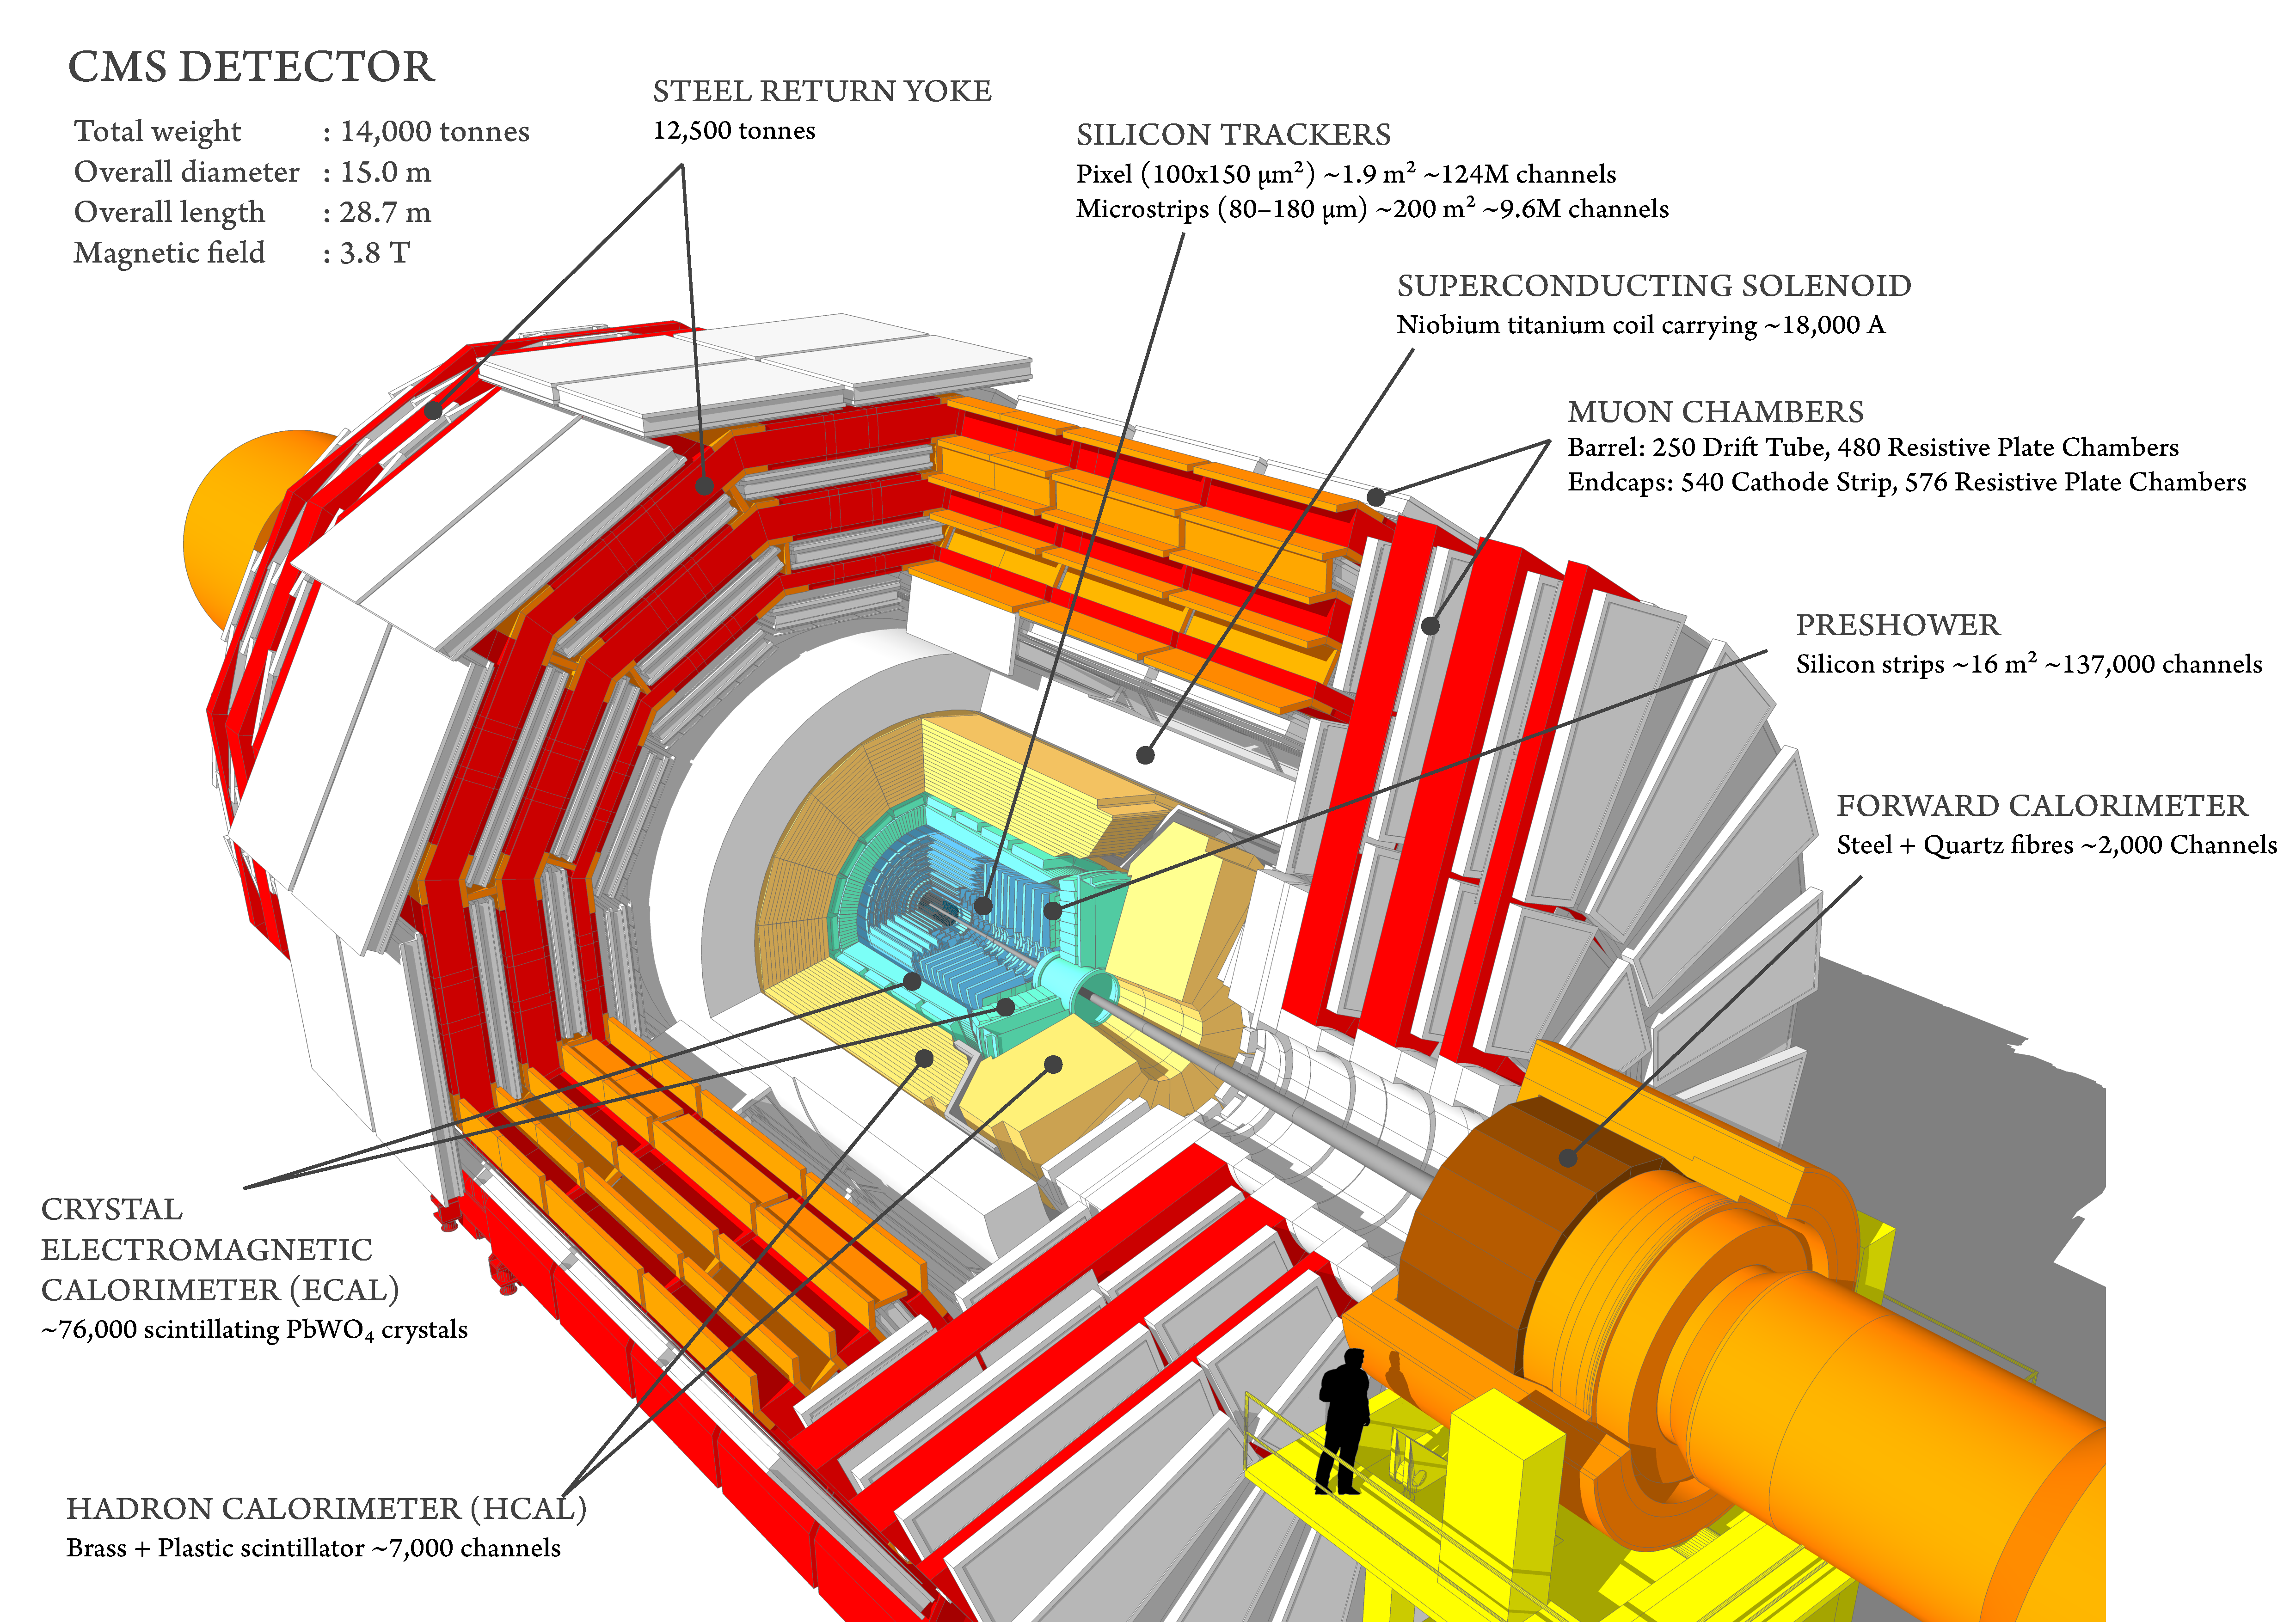
\includegraphics[width=\textwidth]{figures/cms_cutway_ME4_2.pdf}
  \caption[The CMS detector cutaway view]%
  {The CMS detector cutaway view~\cite{image-cms-cutway}}%
  \label{fig:cms-cutaway}
\end{figure}

Figure~\ref{fig:cms-slice} shows a schematic view of the \gls{CMS} detector, and
how different particles leave signature in various sub-detectors.
Neutral particles such as photons, neutrinos, and neutral hadrons will leave no track
in the \gls{ST}, and are identified only by the energy deposited
in the calorimeters or the missing energy in an event.
Electrons are identified from the track in the \gls{ST} and energy deposit
in the \gls{ECAL}. Since hadrons are heavier and they pass through the \gls{ECAL}
and deposit their most of energy in the \gls{HCAL}, leaving only small fraction
of energy in the \gls{ECAL}.
Since muons are \glspl{MIP}, they pass through whole detector with very small
fraction of the energy deposited in the \gls{ECAL} and \gls{HCAL}.

This following section gives an overview of the subsystems of \gls{CMS} detector.
For detailed technical description refer to~\cite{CMS-JINST-S08004}.

\begin{figure}[!ht]
  \centering
  \includegraphics[width=\textwidth]{figures/cms_slice.png}
  \caption[Schematic view of the CMS detector]%
  {Schematic view of the CMS detector~\cite{image-cms-slice}}%
  \label{fig:cms-slice}
\end{figure}

\clearpage{}
\subsection{
  The CMS Coordinate System
}\label{ch_cms:cms-coordinate}

CMS uses \gls{IP} of the collisions as origin to define the right-handed
coordinate system. The \( z \)-axis is along the beamline,
the \( x \)-axis points toward the center of the \gls{LHC},
and the \( y \)-axis points upwards toward the Earth's surface.
The transverse plane \( x - y \) is used to calculate
most commonly used quantities like transverse momentum \( p_{T} \)
and energy \( E_{T} \).

To describe the direction of particles leaving the \gls{IP},
azimuthal \( \phi \) and polar \( \theta \) angles are used.
\( \phi \) is measured around the beam axis,
and \( \theta \) is measured from the beam axis.
In collider physics, pseudorapidity \( \eta \) (Lorentz invariant) is used
to describe direction from beam pipe instead of \( \theta \) as,
%
\begin{equation}
  \eta = - \ln[\tan{\theta/2}]
\end{equation}

and sometimes in terms of rapidity \( y \) as,
%
\begin{equation}
  y = \frac{1}{2} \ln{\frac{E+p_{z}}{E-p_{z}}}
\end{equation}

Particle kinematics can be completely described in terms of
\( p_{T} \), \( \eta \), \( \phi \), and \( E_{T} \) or mass.
The distance between the two particles in \( \eta - \phi \) plane
is described as \( \Delta R \),
%
\begin{equation}
  \Delta R = \sqrt{ {(\Delta \eta)}^{2} + {(\Delta \phi)}^{2} }
\end{equation}

\subsection{
  The Superconducting Magnet
}

The superconducting magnet is the central part of the \gls{CMS} detector, it is
12.5 meters long and 6.3 meters in diameter. The magnet is cooled to
4.5\,\text{K}\xspace and a 20\,\text{kA}\xspace current flows through it to
generate 3.8\Tesla{} of magnetic field with stored energy of 2.6\,\text{GJ}\xspace.

Figure~\ref{fig:cms-magnet} shows the
installation (in 2007) of the superconducting magnet with iron yoke in the underground
cavern.

The key purpose of the magnet is to help determine the momentum and the sign of charged
particles by bending them. The momentum resolution of the particles
decreases with increase in their \(p_T \). Constant magnetic field of 3.8\Tesla{}
gives momentum resolution of \(\Delta p /p \approx 10 \% \). This resolution
is enough to determine unambiguously the sign of muons with
momentum of \(\approx 1\TeV{}/c \).

\begin{figure}[!ht]
  \centering
  \includegraphics[width=0.75\textwidth]{figures/cms_magnet_lowered.jpg}
  \caption%
  [The picture of the CMS detector central part when lowered in underground
    cavern with superconducting magnet and iron
    yoke]%
  {The picture of the CMS detector central part when lowered in underground
    cavern with superconducting magnet and iron
    yoke~\cite{image-cms-magnet}.}%
  \label{fig:cms-magnet}
\end{figure}


\subsection{
  The Tracking System
}

The \gls{CMS} tracking system \gls{ST} is the innermost part of the detector, it
is made up of pixel and strip detectors. The main goal of \gls{ST} is to
reconstruct the tracks of the charged particles with high precision in high pileup
environment.

Silicon is most commonly used material for making tracking systems because of it's
semiconductor properties, and high radiation hardness which is essential for the
innermost detector. When a p-n junction is built on silicon substrate it creates
a depletion zone with no charge carriers at the junction, and whenever
a charged particle passes through the depletion zone it creates a electron-hole pair.
Under reverse bias this electron-hole generates an electrical signal. The \gls{CMS}
tracker consists of about 124 million channels of such junctions in the
pixel detector and 10 million in the strip detector.

The pixel detector was upgraded in 2017 and the comparison of layers before
and after the upgrade is shown in Figure~\ref{fig:cms-pixel}. It is made up of
four barrel layers and three endcaps, with nearest barrel layer being 3\cm{}
away from the beamline for precise measurement of the \gls{IP}.
Because of the large number of pixel channels, the readout is done by \glspl{ASIC}.

\begin{figure}[!ht]
  \centering
  \begin{minipage}[c]{.62\textwidth}
    \includegraphics[trim={80pt 0 80pt 0},clip,width=\textwidth]%
    {figures/cms_pixel_phase1.pdf}
  \end{minipage}
  \begin{minipage}[c]{.35\textwidth}
    \includegraphics[width=\textwidth]{figures/cms_pixel_phase1_04.png}
  \end{minipage}
  \caption[The CMS pixel upgrade]%
  {The CMS pixel upgrade. The left is cross sectional view of pixel detector
    layers before upgrade (bottom) and after Phase 1 upgrade (top).
    The right is view pixel barrel before upgrade (left)
    and after upgrade (right)~\cite{image-cms-pixel}.}%
  \label{fig:cms-pixel}
\end{figure}

The outermost part of \gls{ST} detector is made up of silicon strips. It allows for large
coverage by reducing number of readout channels. It has 10 layers in barrel region
and 12 discs in endcap region. For better signal-to-noise ratio and radiation
tolerance both pixel and strip detector are operated at -20\,\de\text{C}\xspace.

\subsection{
  The Electromagnetic Calorimeter
}

The \gls{ECAL} active material is made of lead tungstate (PbWO\textsubscript{4})
scintillating crystals and two layers silicon strip for preshower
in front of the endcaps. The crystals in central barrel section are mounted
in quasi-projective geometry pointing towards \gls{IP} and cover
\( |\eta| < 1.48 \). The two endcaps extends the coverage to
\( |\eta| = 3.0 \). The schematic layout of \gls{ECAL} is shown in Figure~\ref{fig:cms-ecal-schematic}
and the picture of endcap quadrant when assembled is shown in Figure~\ref{fig:cms-ecal-ee}

The main purpose of the \gls{ECAL} is to determine energy and positions of
electromagnetically interacting particles.
Except electron and photons all other particles pass
through \gls{ECAL} crystals with only small fraction of energy signature in the crystals.
When electron and photon interacts with PbWO\textsubscript{4} it starts an process
of electromagnetic shower which continues until the energy the energy of the incident
particle is below threshold, which is about 1\MeV{}.

\begin{figure}[!ht]
  \centering
  \begin{minipage}[c]{.60\textwidth}
    \includegraphics[width=\textwidth]{figures/cms_ecal_schematic.pdf}
  \end{minipage}
  \begin{minipage}[c]{.38\textwidth}
    \includegraphics[width=\textwidth]{figures/cms_ecal_layout.png}
  \end{minipage}
  \caption[The CMS \gls{ECAL} schematic layout]%
  {The \gls{CMS} \gls{ECAL} schematic layout. The left schematic shows the arrangement of
    superclusters in barrel and endcap (with preshower layers). On the right is the \(y-z \)
    plane quarter view of \gls{ECAL} layout~\cite{image-cms-ecal-layout}.}%
  \label{fig:cms-ecal-schematic}
\end{figure}

\begin{figure}[!ht]
  \centering
  \includegraphics[width=0.60\textwidth]{figures/cms_ecal_ee_quadrant.jpg}
  \caption[The \gls{ECAL} endcap quadrant assembled view]%
  {The \gls{ECAL} endcap quadrant assembled view~\cite{image-cms-ecal-ee-quadrant}.}%
  \label{fig:cms-ecal-ee}
\end{figure}

The fractional resolution of the \gls{ECAL} energy measurements can be described as,
%
\begin{equation}
  {\left( \frac{\sigma}{E} \right)}^2
  = {\left( \frac{S}{\sqrt{E}} \right)}^2
  + {\left( \frac{N}{E} \right)}^2
  + C^2
\end{equation}

where \(S \) is the stochastic term, \(N \) is related to the noise,
and C is a constant offset. The energy resolution in the central
region of \gls{ECAL} barrel (\( |\eta| < 0.8 \)) for electrons from \textit{Z}
decays was 2\% and 2--5\% elsewhere. The energy resolution for photons
from Higgs decay varied from 1.1\% to 2.6\% in the barrel region and
from 2.2\% to 5\% in the endcaps~\cite{energy-ecal-7tev}.

\subsection{
  The Hadronic Calorimeter
}

Similar to \gls{ECAL}, the purpose of \gls{HCAL}
is to shower hadrons, and measure their energy and position.
The first half of barrel \gls{HCAL} inserted into solenoid during installation
is shown in Figure~\ref{fig:cms-hcal-inserted}.

\gls{HCAL} is made up of
towers pointing towards \gls{IP} where each tower is made up of sampling layers;
with alternating layers of plastic scintillator and brass.
Brass acts as absorber in the \gls{HCAL} and causes hadrons to shower.
Scintillators emits light when secondary particles
from hadronic shower pass through them.
The light output collected from the scintillator layers, combined with
total absorption length of Brass layers
gives the total energy deposited in the \gls{HCAL}.
In phase 1 upgrade the \gls{HCAL} was upgraded
to give energy deposit as a function of depth.
The depth segmentation schematic is
show in Figure~\ref{fig:cms-hcal-depth} and the details of upgrade are in technical design
report~\cite{cms-hcal-upgrade}.

\begin{figure}[!ht]
  \centering
  \includegraphics[width=\textwidth]{figures/cms_hcal_hb_inserted.jpg}
  \caption[The first half of the barrel \gls{HCAL} inserted into the
    superconducting solenoid (April 2006)]%
  {The first half of the barrel \gls{HCAL} inserted into the
    superconducting solenoid (April 2006)~\cite{image-cms-hcal-inserted}.}%
  \label{fig:cms-hcal-inserted}
\end{figure}

\gls{HCAL} consists barrel (HB) and two endcaps (HE) located inside solenoid.
These two subsystems combined provides
coverage of \( |\eta| \le 3.0 \).
There are two other subsystems of \gls{HCAL} outside solenoid,
a forward \gls{HCAL} (HF) and outer barrel \gls{HCAL} (HO).
HO was added to ensure there is no leakage from the particles that
make it past the solenoid. HF extends the coverage
to \(|\eta| \le 5.0\). HF is based on Cherenkov radiation principle
and uses quartz fiber as active material with steel absorbers.

\begin{figure}[!ht]
  \centering
  \includegraphics[width=\textwidth]{figures/cms_hcal_depth_seg.pdf}
  \caption[The \gls{HCAL} depth segmentation after phase 1 upgrade]%
  {The \gls{HCAL} depth segmentation after phase 1 upgrade~\cite{image-cms-hcal-depth}.}%
  \label{fig:cms-hcal-depth}
\end{figure}

\subsection{
  Muon Detector
}

The outermost subsystem in the \gls{CMS} detector is the muon detector.
Unlike electrons, muons are \glspl{MIP} i.e.
they do not lose much of their energy
while passing through tracker, calorimeter and solenoid.
Muon detector is built to identify, measure momentum and trigger the events
with muons. Like other subsystems, the muon detector consists of a barrel and endcap
detector. The schematic layout is highlighted in the Figure~\ref{fig:cms-muon-system}.
As shown in the schematic, the muon detector consists of three subsystems \glspl{DT}, \glspl{CSC} and
\glspl{RPC}.

The \glspl{DT} are wire gas detectors filled with Argon and composed of
many tube cells of about 4\cm{}. Muon passing through these tubes
ionize Argon and the free electron is detected on the wire cathode.
Each DT is about 2 meters by 2.5 meters in size, and there are four layers
of the \glspl{DT} interleaved with the iron yoke, parallel to
the beam pipe in barrel region. The drift time is the order of about 380\nanoseconds.

\begin{figure}[!ht]
  \centering
  \includegraphics[width=0.9\textwidth]{figures/cms_muon_system.pdf}
  \caption[The quadrant view of CMS subdetectors layout, and
    the coverage of the muon detector \glspl{DT}, \glspl{CSC},
    and \glspl{RPC} highlighted]%
  {The quadrant view of CMS subdetectors layout, and
    the coverage of the muon detector \glspl{DT}, \glspl{CSC},
    and \glspl{RPC} highlighted~\cite{image-cms-muon-system}.}%
  \label{fig:cms-muon-system}
\end{figure}

The \glspl{CSC} are based on same principle as \glspl{DT},
and are made of multi-wire proportional chambers consisting of
6 anode planes interleaved with 7 cathode planes. They have time resolution
better than 5\nanoseconds. The \glspl{CSC} are used in endcap region,
where radiation hardness is required, and non uniform magnetic field does not
effects the measurement.

The \glspl{RPC} are made up of two oppositely charged high resistive parallel
plates with a gas\footnote{mixture of 96.2\% \( C_{2}H_{2}F_{4} \), 3.5\% Iso-\( C_{4}H_{10} \),
0.3\% \( S{F}_{6} \)} volume between them.
When a charged particles passes through, it ionizes the gas, and it creates
an avalanche. The charge is collected by metallic readout strips.
\glspl{RPC} have poor position resolution but fast readout of the order of 1\nanoseconds,
which is fast compared to \glspl{DT}, this is the reason there are 1 or 2 \glspl{RPC}
attached to both \glspl{DT}, and \glspl{CSC}.

\subsection{
  Trigger
}\label{ch_cms:L1T}

Since proton-proton collisions occurs every bunch crossing which are
25\nanoseconds{} apart; equivalent to a 40\,\text{MHz}\xspace collisions rate.
At this collisions rate, the data storage required will be enormous
and \gls{CMS} can only record up to 1000 events per second. Since most of events
do not contain interesting physics events, they can be thrown away.
To do this \gls{CMS} has two tier trigger system \gls{L1T}, and \gls{HLT}.

The \gls{L1T} is the first electronic processing system through
which event information is processed before it is passed to
second trigger system: \gls{HLT}.
The \gls{L1T} is designed to make fast decisions in about 3.8\mus,
and only uses \gls{ECAL}, \gls{HCAL} and muon system to make a decision
regarding throwing or keeping an event.
\gls{L1T} cut downs the data rate from 40\,\text{MHz}\xspace to
100\,\text{kHz}\xspace. The \gls{L1T} electronics is placed next to
the detector in underground cavern for fast transfer of data.

Events accepted by \gls{L1T} are passed to the \gls{HLT}.
The \gls{HLT} further reduces the data rate from 100\,\text{kHz}\xspace to
about 1\,\text{kHz}\xspace using a computer farm with nearly 26000 cores.
\gls{HLT} uses all the available information from the event to make
decision in about 300 ms. \gls{HLT} is modular by design
to allow the use of information from different systems to construct
multiple paths called \gls{HLT} paths, for example the single muon \gls{HLT}
path will save event with at least one muon passing the selection criteria
set in \gls{HLT} path. Events passing at least on \gls{HLT} path are
saved for offline physics analysis.
